\chapter{Background and Related Work}
\label{chap:background}

\section{Literature Review}

Automated citation verification builds on three established areas of software engineering and natural language processing (NLP): scholarly document parsing, bibliographic record linkage, and hallucination detection. This section reviews representative approaches in each area and compares existing tools against \textbf{CITRA}.

\subsection{Document Parsing and Reference Extraction}

Extracting structured citations from unlabeled PDF files is the first stage of any bibliography checker. Errors introduced during parsing propagate to every downstream module. The standard open-source engine for scientific PDF segmentation is GROBID~\cite{Lopez2009}, which uses linear-chain Conditional Random Fields (CRFs) to convert raw PDF pages into Text Encoding Initiative XML (\texttt{TEI-XML}) documents containing body paragraphs, inline \texttt{<ref type="bibr">} markers, and structured \texttt{<biblStruct>} entries. Although GROBID performs strongly on typeset journal articles, student capstone reports exported from word processors often contain multi-line tables of contents, inconsistent indentation, or Vietnamese legal citations that pure CRF models misclassify or truncate.

When structural tags are absent, layout-aware PDF parsers provide a vital fallback. PyMuPDF~\cite{PyMuPDF2024} extracts text blocks rapidly through compiled C bindings, whereas \texttt{pdfplumber}~\cite{Pdfplumber2024} exposes character-level coordinates needed to reconstruct two-column page layouts and hanging indents. \textbf{CITRA} combines GROBID \texttt{0.9.1-crf} with deterministic table-of-contents filtering, regular-expression field enrichment, PyMuPDF/\texttt{pdfplumber} fallback, and native \texttt{python-docx} parsing so that malformed student formatting does not halt verification.

\subsection{Bibliographic Record Linkage}

Record linkage determines whether two noisy metadata records refer to the same real-world publication. Fellegi and Sunter~\cite{Fellegi1969} established the probabilistic foundation for entity resolution by showing that combining multiple independent field comparisons (title, author surname, publication year, and venue) yields much lower error rates than matching a single concatenated string. Equally important is asymmetric negative evidence: a direct contradiction between two populated fields (such as a valid DOI resolving to an unrelated title) provides strong proof that a citation is corrupted, whereas a missing venue field merely lowers confidence. This distinction motivates \textbf{CITRA}'s priority-ordered rule hierarchy, which evaluates explicit identifier and retraction contradictions before scoring partial metadata similarity.

\subsection{Hallucinated Citation Detection versus AI-Text Attribution}

Recent responses to LLM misuse in education follow two fundamentally different paradigms, as contrasted in Figure~\ref{fig:verification-paradigm}. The first paradigm, \emph{stylistic attribution}, trains statistical classifiers or watermark detectors to estimate the probability that prose was generated by an AI model~\cite{Sculley2015}, \cite{Goodfellow2016}. However, Sadasivan et al.~\cite{Sadasivan2023} proved theoretically and empirically that paraphrasing drives stylometric detector accuracy toward random guessing. Krishna et al.~\cite{krishna2023paraphrasing} confirmed that discourse-level paraphrasing evades commercial and watermark-based AI detectors while demonstrating that retrieval-grounded verification remains robust. Furthermore, stylometric detectors inspect only surface token distributions; they cannot tell whether a cited paper actually exists, and class imbalance in real student cohorts inflates false-positive rates~\cite{Chawla2009}.

\begin{figure}[H]
    \centering
    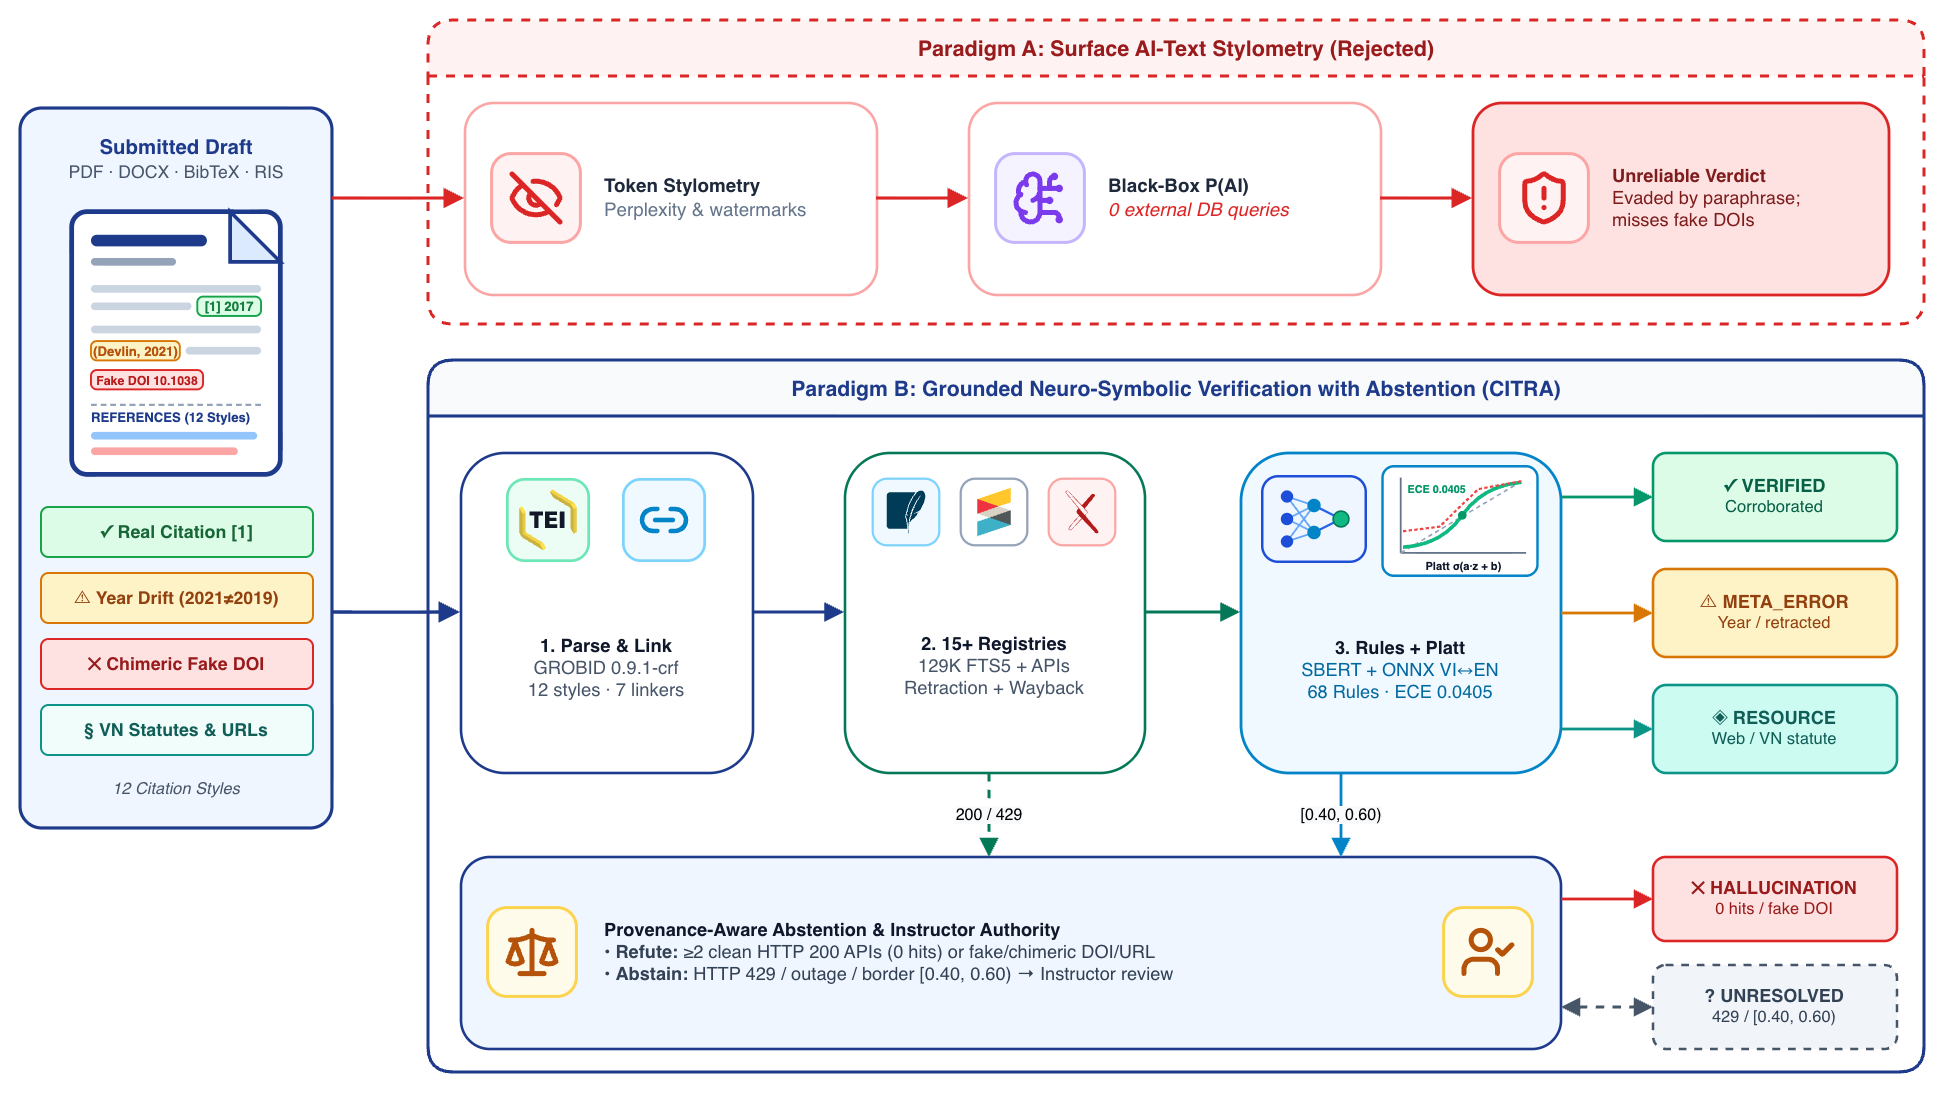
\includegraphics[width=\textwidth,keepaspectratio]{picture/figures/fig2_1_verification_paradigm.png}
    \caption[Comparison between stylistic attribution and external bibliographic verification]{Comparison between stylistic attribution of machine-generated text and external bibliographic verification with provenance-aware abstention.}
    \label{fig:verification-paradigm}
\end{figure}

The second paradigm, \emph{external bibliographic and claim verification}, checks each citation against authoritative registries and compares inline claims against retrieved evidence, following fact-verification frameworks such as FEVER~\cite{thorne2018fever}, SciFact~\cite{wadden2020scifact}, and citation-grounded generation benchmarks such as ALCE~\cite{gao2023alce}. Every flag raised under this paradigm points to concrete external evidence: either multiple live registries confirm that no matching record exists, or a retrieved canonical record exposes a specific metadata or claim discrepancy.

\subsection{Comparison with Existing Systems}

Existing academic integrity platforms, reference managers, and research benchmarks each address only part of the student manuscript verification workflow. Plagiarism checkers such as Turnitin match text overlap against closed repositories but do not detect fabricated references that have zero text overlap with existing literature. Reference managers such as Zotero import clean DOIs for authors but do not audit in-text citation consistency or classroom cohorts. Closed-corpus NLP benchmarks such as SciFact~\cite{wadden2020scifact} verify scientific claims over a fixed set of 5,000 abstracts but do not parse multi-style PDFs or query live registries. Table~\ref{tab:related-work} compares \textbf{CITRA} against five representative system categories across seven technical capabilities.

{\setlength{\tabcolsep}{3.5pt}
\begin{longtable}{|L{0.22}|C{0.11}|C{0.11}|C{0.11}|C{0.12}|C{0.11}|C{0.11}|C{0.11}|}
\caption{Feature comparison between existing tool categories and CITRA (\texttt{v3.90.5}).}\label{tab:related-work}\\
\hline
\textbf{System Category} & \textbf{Multi\-Style PDF} & \textbf{Bipar\-tite Linker} & \textbf{15+ Live APIs} & \textbf{Claim Align.} & \textbf{Safe Abstain} & \textbf{Calib.\ Prob.} & \textbf{VN Legal} \\
\hline
\endfirsthead
\multicolumn{8}{c}{\itshape Table \thetable\ (continued from previous page)}\\
\hline
\textbf{System Category} & \textbf{Multi\-Style PDF} & \textbf{Bipar\-tite Linker} & \textbf{15+ Live APIs} & \textbf{Claim Align.} & \textbf{Safe Abstain} & \textbf{Calib.\ Prob.} & \textbf{VN Legal} \\
\hline
\endhead
\hline
\multicolumn{8}{r}{\itshape Continued on next page}\\
\endfoot
\hline
\endlastfoot
Text Overlap Tools (Turnitin / iThenticate) & Partial & No & No & No & No & No & No \\
\hline
AI Style Detectors (GPTZero / Watermarks) & No & No & No & No & No & Partial & No \\
\hline
Prompt-Only LLM Checkers & Partial & No & Partial & Partial & No & No & No \\
\hline
Reference Managers (Zotero / GROBID) & Yes & No & Partial & No & No & No & No \\
\hline
Claim Benchmarks (SciFact / ALCE) & No & No & No & Yes & Partial & No & No \\
\hline
\textbf{CITRA (\texttt{v3.90.5})} & \textbf{Yes (12)} & \textbf{Yes (8)} & \textbf{Yes (15+)} & \textbf{VI$\leftrightarrow$EN} & \textbf{Yes} & \textbf{Platt} & \textbf{Yes} \\
\hline
\end{longtable}
}

\section{Scholarly Registries and Persistent Identifiers}

\subsection{Federated Bibliographic Sources}

Large-scale bibliometric studies show substantial coverage gaps between individual scholarly databases across disciplines and publication types~\cite{visser2021bibliographic}. Relying on a single API also creates severe rate-limit bottlenecks during classroom submission deadlines. \textbf{CITRA} therefore combines an offline full-text corpus with domain-aware routing across more than fifteen scholarly, technical, and archival registries, as summarized in Table~\ref{tab:sources}.

\begin{longtable}{|L{0.27}|L{0.36}|L{0.37}|}
\caption{Scholarly registries and validators integrated into the CITRA retrieval layer.}\label{tab:sources}\\
\hline
\textbf{Source / Validator} & \textbf{Primary Coverage} & \textbf{Role in Pipeline} \\
\hline
\endfirsthead
\multicolumn{3}{c}{\itshape Table \thetable\ (continued from previous page)}\\
\hline
\textbf{Source / Validator} & \textbf{Primary Coverage} & \textbf{Role in Pipeline} \\
\hline
\endhead
\hline
\multicolumn{3}{r}{\itshape Continued on next page}\\
\endfoot
\hline
\endlastfoot
\textbf{Local Corpus} (\texttt{local\_papers.db}) & \textbf{129,125 records} (128,105 unique papers; 82,877 abstracts) from ACL Anthology~\cite{acl-anthology} and arXiv & \textbf{Tier 0} sub-100\,ms offline SQLite FTS5 BM25 lookup \\
\hline
\textbf{Seminal Whitelist} (\texttt{\_KNOWN\_PAPERS}) & \textbf{101} foundational CS, AI, NLP, and deep learning publications & \textbf{Tier 0} instant lookup for heavily cited canonical papers \\
\hline
\textbf{Crossref}~\cite{crossref-tdm} \& \textbf{Retraction Watch} & Peer-reviewed journals, proceedings, book chapters, and retraction notices & \textbf{Tier 1} DOI resolution, Journal Article Tag Suite (JATS) abstract parsing, and \texttt{is\_retracted} screening \\
\hline
\textbf{OpenAlex}~\cite{openalex} & Global open scholarly graph spanning journals, preprints, and repositories & \textbf{Tier 1} broad metadata lookup and inverted-index abstract reconstruction \\
\hline
\textbf{DataCite}~\cite{datacite} \& \textbf{Global DOI RA}~\cite{doi-handbook} & Zenodo/Figshare/OSF datasets and regional DOI agencies (JaLC, CNKI, KISTI, mEDRA) & \textbf{Tier 1} non-Crossref DOI resolution and \texttt{R-DOI-RA-NO-CSL} safe abstention \\
\hline
\textbf{DOAJ}~\cite{doaj} \& \textbf{OpenAIRE / HAL} & Open-access journals (including regional Asian venues), institutional repositories, and preprints & \textbf{Tier 1} open-access journal and institutional repository verification \\
\hline
\textbf{DBLP}~\cite{dblp} \& \textbf{arXiv API}~\cite{arxiv-api} & Computer science conferences/workshops and STEM preprints & \textbf{Tier 1} domain-routed CS/AI bibliography and exact \texttt{arXiv} ID lookup \\
\hline
\textbf{Europe PMC}~\cite{europepmc} \& \textbf{NCBI / bioRxiv} & PubMed/MEDLINE biomedical, clinical, psychology, and life-science preprints & \textbf{Tier 1} domain-routed life-science lookup and abstract enrichment \\
\hline
\textbf{OpenLibrary}~\cite{openlibrary} \& \textbf{Google Books} & Textbooks, monographs, ISBN metadata, and multi-edition printings & \textbf{Tier 1} book verification and cross-edition year tolerance \\
\hline
\textbf{Hugging Face, IETF RFC, PyPI \& Wikidata} & ML models/datasets, RFC internet standards, Python packages, and OpenCitations & \textbf{Tier 1} software, technical standard, and open citation verification \\
\hline
\textbf{Serper / SerpAPI Router} & Academic web index fallback & \textbf{Tier 2} optional fallback when Tier 0 and Tier 1 return zero candidates \\
\hline
\textbf{HTTP + Wayback} \texttt{Link\allowbreak Validator}~\cite{openlibrary} & Live HTTP/HTTPS targets and Internet Archive CDX snapshots & \textbf{Parallel} URL liveness, Soft-404 HTML metadata, and archive check \\
\hline
\end{longtable}

\subsection{DOI Resolution and Retraction Screening}

A Digital Object Identifier (DOI) provides a persistent handle for scholarly objects~\cite{doi-handbook}, yet syntactic validity (\texttt{10.xxxx/...}) does not guarantee legitimacy. Generative models frequently invent unregistered suffixes under real publisher prefixes (such as \texttt{10.1109/}) or copy a real DOI from a high-profile paper onto a fabricated citation. Conversely, legitimate Asian or European journals registered through agencies such as JaLC, CNKI, KISTI, or mEDRA resolve at \texttt{doi.org/ra/} without exposing metadata in Crossref. Querying the Global DOI Registration Agency API allows \textbf{CITRA} to abstain safely on valid regional DOIs while exposing unregistered and chimeric DOIs. Simultaneously, checking Crossref update-to metadata and Retraction Watch flags prevents retracted articles from passing silently as verified sources.

\section{Theoretical Foundations}

\subsection{Lexical and Semantic Title Similarity}

Bibliographic strings vary across citation styles due to subtitle truncation, punctuation differences, hyphenation, and edition markers. \textbf{CITRA} therefore combines lexical string similarity with dense neural embeddings. At the lexical level, RapidFuzz computes token-set ratios (insensitive to word reordering), normalized Levenshtein ratios (sensitive to character typos), and guarded prefix ratios (handling omitted subtitles after colons). At the semantic level, titles are encoded into 384-dimensional vectors using the Transformer architecture~\cite{vaswani2017} distilled via BERT~\cite{bert} and MiniLM~\cite{wang2020minilm} into the Sentence-BERT checkpoint \texttt{all-MiniLM-L6-v2}~\cite{reimers2019sbert}. When Vietnamese prose cites an English source, \textbf{CITRA} activates a quantized ONNX INT8 multilingual encoder (\texttt{paraphrase-multilingual-MiniLM-L12-v2}) trained via multilingual knowledge distillation~\cite{reimers2020multilingual}.

\subsection{Multi-Sentence Context Alignment}

Checking bibliography metadata alone cannot catch \emph{contextual misattribution}, where a student cites a real paper to support an unrelated or opposite claim. However, comparing a single in-text sentence directly against an entire ten-sentence abstract suffers from length dilution because background and conclusion sentences wash out the specific sentence being cited. Given an in-text citation context $c$ and a candidate abstract $A$ segmented into sentences $\{s_1, \dots, s_m\}$, \textbf{CITRA} computes the pooled abstract alignment score $s_{\text{abs}}(c, A)$ defined in Equation~\eqref{eq:abs-pooling}:
\begin{equation}\label{eq:abs-pooling}
s_{\text{abs}}(c, A) = \max\Bigl(\cos\bigl(\mathbf{e}(c), \mathbf{e}(A)\bigr),\; 0.65 \max_{1 \le i \le m} \cos\bigl(\mathbf{e}(c), \mathbf{e}(s_i)\bigr) + 0.35 \cos\bigl(\mathbf{e}(c), \mathbf{e}(A)\bigr)\Bigr),
\end{equation}
where $\mathbf{e}(\cdot)$ denotes the L2-normalized sentence embedding. Equation~\eqref{eq:abs-pooling} preserves high similarity when a citation targets a single specific finding while retaining whole-abstract context when a citation summarizes the overall paper. The final content alignment combines title similarity ($0.30$), pooled abstract similarity ($0.50$), and full-text snippet similarity ($0.20$, renormalized when full text is absent).

\subsection{Selective Classification and Logit-Space Platt Calibration}

In high-stakes decision support, a classifier must know when to abstain~\cite{chow1970optimum}, \cite{Geifman2017}, and its reported confidence $p$ must match empirical accuracy~\cite{hand2009}, \cite{guo2017}. Static rule confidences cluster at discrete constants and overestimate certainty near decision boundaries. Given the symbolic verdict class $y_{\text{sym}}$ and the 16-dimensional feature vector $\mathbf{x} \in \mathbb{R}^{16}$, \textbf{CITRA} blends the symbolic rule confidence $C_{\text{sym}}$ with the predicted class probability $P_{\text{ML}}(y_{\text{sym}} \mid \mathbf{x})$ of a Multinomial Logistic Regression model using weight $\alpha \in [0, 1]$, as defined in Equation~\eqref{eq:platt-calib}:
\begin{equation}\label{eq:platt-calib}
p_{\text{blend}} = \alpha C_{\text{sym}} + (1 - \alpha) P_{\text{ML}}(y_{\text{sym}} \mid \mathbf{x}), \;\;
P_{\text{cal}} = \operatorname{clip}\!\left(\sigma\Bigl(a \cdot \ln\frac{\tilde{p}}{1 - \tilde{p}} + b\Bigr),\, 0.01,\, 0.99\right),
\end{equation}
where $\tilde{p} = \min(\max(p_{\text{blend}}, 10^{-4}), 1 - 10^{-4})$ prevents numerical overflow at $0$ or $1$, $\sigma(z) = (1 + e^{-z})^{-1}$ is the logistic sigmoid, and $(a, b)$ are scalar Platt scaling parameters~\cite{platt1999} fitted on a disjoint validation split by minimizing a joint negative log-likelihood and Brier score objective~\cite{brier1950}.

\subsection{Paper-Disjoint Evaluation Design}

Following Empirical Software Engineering experimentation guidelines~\cite{wohlin2012experimentation} and claim-verification benchmarks~\cite{thorne2018fever}, \cite{wadden2020scifact}, training and evaluating a hybrid verifier requires strict protection against data leakage and dataset artifacts~\cite{gururangan2018annotation}, \cite{poliak2018hypothesis}. If perturbed variants of the same base paper appear in both training and testing splits, a classifier can memorize paper-level feature distributions. Similarly, if non-zero semantic context scores appear only in verified examples, the model learns a trivial shortcut. All quantitative experiments in Chapter~\ref{chap:results} therefore partition base papers strictly before perturbation, retain real Sentence-BERT encodings across all classes without artificial clamping, and evaluate hypotheses using continuity-corrected McNemar tests~\cite{dietterich1998approximate}, Holm--Bonferroni multiple-comparison adjustments~\cite{holm1979simple}, and paired bootstrap resampling~\cite{bergkirkpatrick2012empirical}, \cite{dror2018hitchhiker}.

\section{Chapter Summary}

This chapter reviewed the literature on PDF citation parsing, probabilistic record linkage, and hallucinated reference detection, and contrasted \textbf{CITRA} against five categories of existing tools. It also established the multi-registry retrieval rationale and the mathematical formulations for sentence-pooled semantic alignment and logit-space Platt calibration. Chapter~\ref{chap:overview} translates these foundations into formal software requirements, use cases, database schemas, and deployment specifications.
